% Created 2024-02-28 mié 23:39
% Intended LaTeX compiler: pdflatex
\documentclass[bigger]{beamer}
\usepackage[utf8]{inputenc}
\usepackage[T1]{fontenc}
\usepackage{graphicx}
\usepackage{longtable}
\usepackage{wrapfig}
\usepackage{rotating}
\usepackage[normalem]{ulem}
\usepackage{amsmath}
\usepackage{amssymb}
\usepackage{capt-of}
\usepackage{hyperref}
\mode<beamer>{\usetheme{Madrid}}
\usetheme{default}
\author{Adrián Arroyo Calle}
\date{Curso 2023-2024}
\title{Computación paralela y cálculo distribuido}
\hypersetup{
 pdfauthor={Adrián Arroyo Calle},
 pdftitle={Computación paralela y cálculo distribuido},
 pdfkeywords={},
 pdfsubject={},
 pdfcreator={Emacs 29.2 (Org mode 9.6.15)}, 
 pdflang={Spanish}}
\begin{document}

\maketitle

\section{Introducción}
\label{sec:org137aa4e}

\begin{frame}[label={sec:org0c2adfe}]{Contenidos de la asignatura}
\begin{itemize}
\item Introducción
\begin{itemize}
\item Computación paralela y concurrente, sistemas multinúcleo y sistemas distribuidos
\item Rendimiento, escalabilidad y eficiencia
\item Lenguajes
\end{itemize}
\item Estrategias de paralelismo en sistemas multinúcleo
\begin{itemize}
\item Descripción de los sistemas multinúcleo
\item Estrategias, herramientas y modelos de programación paralela
\item Desarrollo de aplicaciones capaces de realizar ejecuciones eficientes en sistemas multinúcleo
\end{itemize}
\item Estrategias de paralelismo en sistemas distribuidos
\begin{itemize}
\item Descripción de los sistemas distribuidos
\item Estrategias, herramientas y modelos para la computación distribuida
\item Desarrollo de aplicaciones capaces de realizar ejecuciones eficientes en sistemas distribuidos
\end{itemize}
\end{itemize}
\end{frame}

\begin{frame}[label={sec:org3f61dab}]{Evaluación}
\begin{block}{Primera convocatoria}
\begin{block}{Porcentajes}
\begin{itemize}
\item Prácticas (40\%)
\begin{itemize}
\item Dos prácticas, 20\% cada una
\end{itemize}
\item Proyecto final (60\%)
\end{itemize}
\end{block}

\begin{block}{Notas mínimas}
\begin{itemize}
\item Nota mínima para superar la asignatura: 5/10
\begin{itemize}
\item Nota mínima en cada práctica: 4/10
\item Nota mínima en el proyecto: 5/10
\end{itemize}
\end{itemize}
\end{block}
\end{block}
\end{frame}

\begin{frame}[label={sec:org962ce32}]{Evaluación II}
\begin{block}{Segunda convocatoria}
\begin{itemize}
\item Un examen sustituye el proyecto final
\item Se mantiene la nota de prácticas (no se puede recuperar)
\item Nota mínima para superar la asignatura: 5/10
\end{itemize}
\end{block}
\end{frame}

\begin{frame}[label={sec:org2674c00}]{Motivación}
¿Por qué es importante la computación paralela y el cálculo distribuido?
\end{frame}

\begin{frame}[label={sec:org869ca0e}]{Motivación II}
\begin{itemize}
\item El microprocesador es el cerebro del ordenador. Ejecuta operaciones aritméticas y de control.
\item Ley de Moore
\begin{quote}
Aproximadamente cada 2 años se duplica el número de transistores en un microprocesador
\end{quote}

\item Desde su creación, la tecnología electrónica sigue avanzando.
\begin{itemize}
\item Se incrementa la capacidad y el rendimiento.

\item Se reduce el coste.
\end{itemize}

\item Una forma de medir el rendimiento es lo que se tarda en ejecutar una tarea.
\end{itemize}
\end{frame}

\begin{frame}[label={sec:org9e22a78}]{Motivación III}
\begin{center}
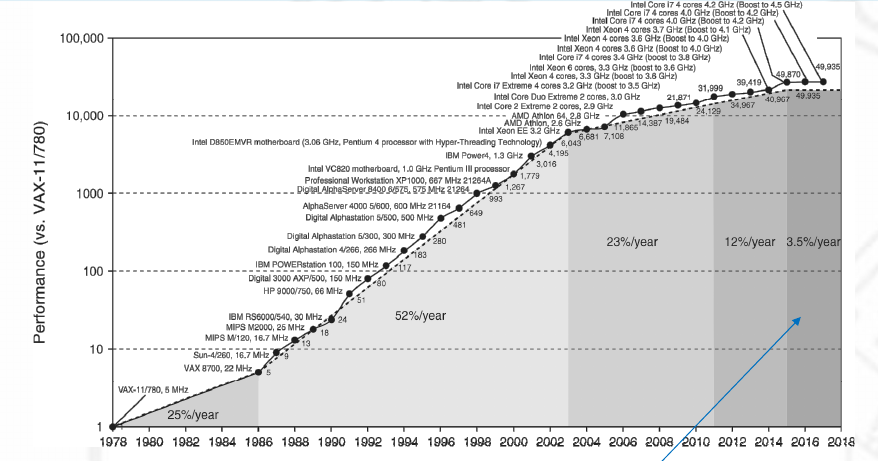
\includegraphics[width=.9\linewidth]{./VUP.png}
\end{center}
\end{frame}

\begin{frame}[label={sec:org22e6585}]{Motivación IV}
¿Por qué cada vez los procesadores cada vez mejoran \alert{menos}?

\begin{itemize}
\item Los procesadores ejecutan sus tareas siguiendo unos ciclos de reloj.
\item Aumentar la frecuencia de los ciclos mejora el rendimiento.
\item Aumentar más la frecuencia es \alert{imposible}.
\end{itemize}
\end{frame}

\begin{frame}[label={sec:org860ff14}]{Muro de Potencia}
\begin{center}
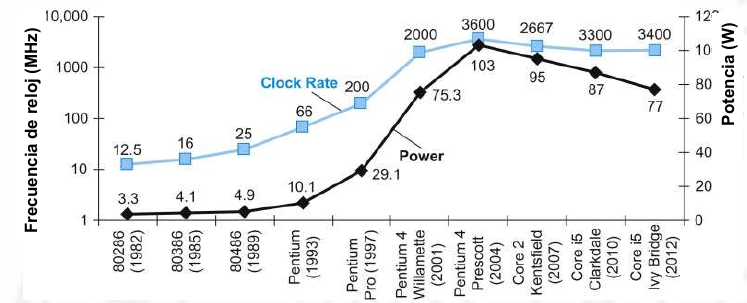
\includegraphics[width=.9\linewidth]{./MuroPotencia.png}
\end{center}
\end{frame}

\begin{frame}[label={sec:org15fb1ef}]{Muro de Potencia II}
\begin{itemize}
\item Aumentar la frecuencia aumenta la potencia necesaria.
\item Aumentar la potencia aumenta la temperatura, que hay que disipar.
\item Se puede reducir el consumo de potencia con más miniaturización (cada vez más complejo, límites físicos) o reduciendo voltaje.
\item Voltajes muy bajos generan pérdidas por corrientes de fuga más elevadas.
\end{itemize}

A este problema se le denomina \alert{muro de potencia}.
\end{frame}

\begin{frame}[label={sec:org64645d6}]{Soluciones}
¿Qué soluciones se pueden plantear?

\begin{itemize}
\item Pipelining de instrucciones
\item Vectorización de instrucciones
\item Optimizar tiempos de espera de I/O
\item Hardware específico para determinadas tareas (GPU, criptografía, \ldots{})
\item Computación cuántica
\item \uline{Procesadores multinúcleo}
\item \uline{Cálculo distribuido}
\end{itemize}

Nos centraremos en las dos últimas
\end{frame}

\begin{frame}[label={sec:orgad9e020}]{¿El santo grial?}
¿Es el procesamiento paralelo el santo grial?

\begin{quote}
Una mujer embarazada a da a luz un bebé tras nueve meses. Si consigo nueve mujeres embarazadas, ¿darán luz a un bebé tras un mes?
\end{quote}

\begin{itemize}
\item No todos los problemas son paralelizables. ¿Cuáles son los impedimentos?
\item Algunos problemas pueden tener un algoritmo paralelo aunque inferior sobre un mononúcleo.
\end{itemize}
\end{frame}

\begin{frame}[label={sec:orgbe61780}]{Julia}
\begin{center}

\includegraphics[width=0.4\textwidth]{./julia.png}
\end{center}

\begin{itemize}
\item Lenguaje de alto rendimiento para aplicaciones científicas.
\item Sintaxis y semántica similar a Python.
\item Pero con rendimiento más cercano a C o FORTRAN.
\item Relativamente reciente
\end{itemize}
\end{frame}

\begin{frame}[label={sec:orgbaef461}]{Descargar Julia}
\url{https://julialang.org/}
\end{frame}

\begin{frame}[label={sec:orga5a24ea}]{Conociendo el ordenador}
\begin{center}
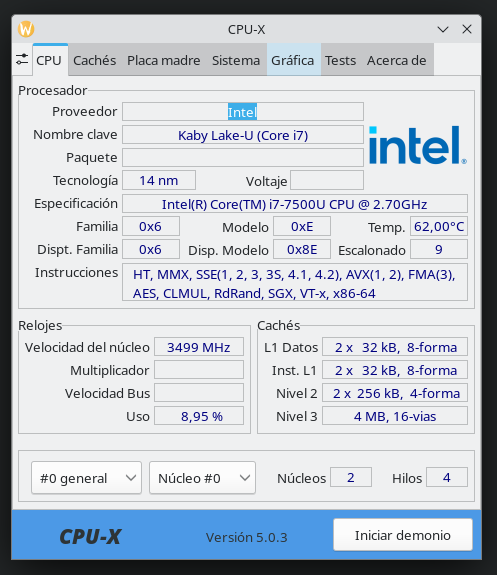
\includegraphics[width=0.4\textwidth]{./CPUX.png}
\end{center}

\begin{itemize}
\item CPU-Z en Windows
\item CPU-X en Linux (/proc/cpuinfo, lscpu, dmidecode, \ldots{})
\end{itemize}
\end{frame}
\end{document}
